\let\lesson\undefined
\newcommand{\lesson}{\phantomlesson{Bài 17.}}
\setcounter{section}{2}
\section{Trắc nghiệm}
\ANSMCQ
{	\begin{center}
		\begin{tabular}{|m{2.8em}|m{2.8em}|m{2.8em}|m{2.8em}|m{2.8em}|m{2.8em}|m{2.8em}|m{2.8em}|m{2.8em}|m{2.8em}|}
			\hline
			1.C  & 2.B  & 3.B  & 4.A  & 5.D  & 6.C  & 7.C  & 8.A  & 9.C  & 10.C  \\
			\hline
		\end{tabular}
	\end{center}
}
\begin{enumerate}[label=\bfseries Câu \arabic*:, leftmargin=1.5cm]
	\item \mkstar{1}\\
	Cơ năng là đại lượng
	\begin{mcq}(2)
		\item luôn luôn dương.
		\item luôn luôn dương hoặc bằng 0.
		\item có thể dương, âm hoặc bằng 0.
		\item luôn luôn khác 0.
	\end{mcq}
\hideall{
\textbf{Đáp án C.}
}

\item \mkstar{1}\\
Một vật được ném thẳng đứng lên cao, khi vật đạt độ cao cực đại thì tại đó
\begin{mcq}(2)
	\item động năng cực đại, thế năng cực tiểu.
	\item động năng cực tiểu, thế năng cực đại.
	\item động năng bằng thế năng.
	\item động năng bằng nửa thế năng.
\end{mcq}
\hideall{
\textbf{Đáp án B.}
}

\item \mkstar{2}\\
Từ độ cao $\SI{5.0}{\meter}$ so với mặt đất, người ta ném một vật khối lượng $\SI{200}{\gram}$ thẳng đứng lên cao với tốc độ đầu là $\SI{2}{\meter/\second}$. Bỏ qua lực cản của không khí. Lấy $g=\SI{10}{\meter/\second^2}$. Xác định cơ năng của vật tại vị trí cao nhất mà vật đạt tới.
\begin{mcq}(4)
	\item $\SI{8.0}{\joule}$.
	\item $\SI{10.4}{\joule}$.
	\item $\SI{4.0}{\joule}$.
	\item $\SI{16.0}{\joule}$.
\end{mcq}
\hideall{
\textbf{Đáp án B.}\\
Do bỏ qua lực cản không khí nên cơ năng của vật bảo toàn:
$$W=\dfrac{1}{2}mv^2_0+mgh=\dfrac{1}{2}\cdot\left(\SI{0.2}{\kilogram}\right)\cdot\left(\SI{2}{\meter/\second}\right)^2+\left(\SI{0.2}{\kilogram}\right)\cdot\left(\SI{10}{\meter/\second^2}\right)\cdot\left(\SI{5}{\meter}\right)=\SI{10.4}{\joule}.$$
}

\item \mkstar{3}\\
{Một con cá heo trong khi nhào lộn đã vượt khỏi mặt biển tới độ cao $\SI{5}{\meter}$. Nếu coi cá heo vượt lên khỏi mặt biển được chỉ nhờ động năng nó có vào lúc rời mặt biển và lấy $g=\SI{10}{\meter/\second^2}$ thì tốc độ của cá heo vào lúc rời mặt biển là
\begin{mcq}(4)
	\item $\SI{10}{\meter/\second}$.
	\item $\SI{7.07}{\meter/\second}$.
	\item $\SI{100}{\meter/\second}$.
	\item $\SI{50}{\meter/\second}$.
\end{mcq}
}
\hideall{
\textbf{Đáp án A.}\\
Áp dụng định luật bảo toàn cơ năng tại vị trí cá heo vừa rời mặt biển và vị trí nó có độ cao cực đại:
$$W_\text{đ1}+W_\text{t1}=W_\text{đ2}+W_\text{t2}\Leftrightarrow \dfrac{1}{2}mv^2_0=mgh_\text{max}$$
$$\Rightarrow v=\sqrt{2gh}=\SI{10}{\meter/\second}.$$
}

\item \mkstar{3}\\
{Một vật khối lượng $\SI{400}{\gram}$ được thả rơi tự do từ độ cao $\SI{20}{\meter}$ so với mặt đất. Cho $g=\SI{10}{\meter/\second^2}$. Sau khi rơi được $\SI{12}{\meter}$, động năng của vật bằng
	\begin{mcq}(4)
		\item $\SI{16}{\joule}$.
		\item $\SI{24}{\joule}$.
		\item $\SI{32}{\joule}$.
		\item $\SI{48}{\joule}$.
	\end{mcq}

}
\hideall{
\textbf{Đáp án D.}\\
Động năng của vật sau khi rơi được $\SI{12}{\meter}$:
$$W_\text{đ}=W-W_\text{t}=mgh_\text{max}-mgh=mgs=\left(\SI{0.4}{\kilogram}\right)\cdot\left(\SI{10}{\meter/\second^2}\right)\cdot\left(\SI{12}{\meter}\right)=\SI{48}{\joule}.$$
}

\item\mkstar{3}\\
Hòn đá được ném thẳng đứng lên với vận tốc $v_0=\SI{20}{\meter/\second}$ từ mặt đất. Chọn gốc thế năng tại mặt đất. Thế năng bằng $\dfrac{1}{4}$ động năng khi vật có độ cao
\begin{mcq}(4)
	\item $\SI{16}{\meter}$.
	\item $\SI{5}{\meter}$.
	\item $\SI{4}{\meter}$.
	\item $\SI{20}{\meter}$.
\end{mcq}
\hideall{
\textbf{Đáp án C.}\\
Áp dụng định luật bảo toàn cơ năng tại vị trí ban đầu và vị trí hòn đá có thế năng bằng $\dfrac{1}{4}$ động năng:
$$W_\text{t}=\dfrac{1}{5}W\Leftrightarrow mgh=\dfrac{1}{5}\cdot\dfrac{1}{2}mv^2_0\Rightarrow h=\SI{4}{\meter}.$$
}

\item\mkstar{3}\\
{Một quả bóng được thả rơi tự do từ độ cao $\SI{20}{\meter}$ so với mặt đất. Khi chạm đất, một phần cơ năng biến thành nhiệt năng nên quả bóng chỉ nảy lên theo phương thẳng đứng với độ cao $\SI{10}{\meter}$. Tỉ số tốc độ của quả bóng trước và sau khi chạm đất bằng
\begin{mcq}(4)
	\item 2.
	\item 0,5.
	\item $\sqrt{2}$.
	\item $\dfrac{1}{\sqrt{2}}$.
\end{mcq}
}
\hideall{
\textbf{Đấp án C.}\\
Tỉ số động năng của quả bóng trước và sau khi chạm đất:
$$\dfrac{W_\text{đ}}{W'_\text{đ}}=\dfrac{mgh}{mgh'}=2$$
$$\Leftrightarrow \dfrac{v^2}{v'^2}=2\Rightarrow v=\sqrt{2}v'.$$
}

\item \mkstar{3}\\
{Từ một đỉnh tháp cao $\SI{20}{\meter}$, người ta ném thẳng đứng lên cao một hòn đá khối lượng $\SI{50}{\gram}$ với tốc độ đầu $\SI{18}{\meter/\second}$. Khi rơi chạm mặt đất, tốc độ của hòn đá bằng $\SI{20}{\meter/\second}$. Lấy $g=\SI{10}{\meter/\second^2}$. Xác định công của lực cản do không khí tác dụng lên hòn đá
	\begin{mcq}(4)
		\item $\SI{-8.1}{\joule}$.
		\item $\SI{-11.9}{\joule}$.
		\item $\SI{-9.95}{\joule}$.
		\item $\SI{-8100}{\joule}$.
	\end{mcq}

}
\hideall{
\textbf{Đáp án A.}\\
Công của lực cản không khí tác dụng lên hòn đá bằng độ biến thiên cơ năng của hòn đá:
\begin{eqnarray*}
A_{F_c}&=&W_2-W_1=\dfrac{1}{2}mv^2_2-\dfrac{1}{2}mv^2_1-mgh\\
&=&\dfrac{1}{2}\cdot\left(\SI{0.05}{\kilogram}\right)\cdot\left[\left(\SI{20}{\meter/\second}\right)^2-\left(\SI{18}{\meter/\second}\right)^2\right]-\left(\SI{0.05}{\gram}\right)\cdot\left(\SI{10}{\meter/\second^2}\right)\cdot\left(\SI{20}{\meter}\right)=\SI{-8.1}{\joule}.
\end{eqnarray*}

}

\item \mkstar{3}\\
{Một con lắc đơn gồm vật nặng khối lượng $m = \SI{400}{\gram}$, dây treo không dãn có chiều dài $\ell=\SI{1.5}{\meter}$. Chọn mốc thế năng tại vị trí cân bằng của vật, lấy $g=\SI{10}{\meter/\second^2}$, ở góc lệch $\alpha=\SI{60}{\degree}$ so với phương thẳng đứng vật có tốc độ $v=\SI{2}{\meter/\second}$. Cơ năng của vật bằng
	\begin{mcq}(4)
		\item $\SI{0.8}{\joule}$.
		\item $\SI{3.0}{\joule}$.
		\item $\SI{3.8}{\joule}$.
		\item $\SI{8.3}{\joule}.$
	\end{mcq}

}
\hideall{
\textbf{Đáp án C.}\\
Cơ năng của con lắc:
\begin{eqnarray*}
W&=&W_\text{t}+W_\text{đ}=mg\ell\left(1-\cos\alpha\right)+\dfrac{1}{2}mv^2\\
&=&\left(\SI{0.4}{\kilogram}\right)\cdot\left(\SI{10}{\meter/\second^2}\right)\cdot\left(\SI{1.5}{\meter}\right)\cdot\left(1-\cos\SI{60}{\degree}\right)+\dfrac{1}{2}\cdot\left(\SI{0.4}{\kilogram}\right)\cdot\left(\SI{2}{\meter/\second}\right)^2=\SI{3.8}{\joule}.
\end{eqnarray*}
}

\item \mkstar{3}\\
{Một con lắc đơn có chiều dài $\ell=\SI{1.6}{\meter}$. Kéo cho dây treo hợp với phương thẳng đứng một góc $\SI{60}{\degree}$ rồi thả nhẹ. Bỏ qua sức cản không khí. Lấy $g = \SI{10}{\meter/\second^2}$. Tốc độ của con lắc khi đi qua vị trí cân bằng là
	\begin{mcq}(4)
		\item $\SI{2.82}{\meter/\second}$.
		\item $\SI{5.66}{\meter/\second}$.
		\item $\SI{4.00}{\meter/\second}$.
		\item $\SI{3.16}{\meter/\second}$.
	\end{mcq}

}
\hideall{
\textbf{Đáp án C.}\\
Áp dụng định luật bảo toàn cơ năng cho con lắc tại vị trí thả và lúc qua vị trí cân bằng (gốc thế năng ở vị trí cân bằng):
$$mg\ell\left(1-\cos\alpha_0\right)=\dfrac{1}{2}mv^2\Rightarrow \left|v\right|=\sqrt{2g\ell\left(1-\cos\alpha_0\right)}=\SI{4}{\meter/\second}.$$
}
\end{enumerate}
\section{Tự luận}
\begin{enumerate}[label=\bfseries Câu \arabic*:, leftmargin=1.5cm]
		\item \mkstar{2}
	
	
	{
		Người ta ném một quả bóng có khối lượng $m=\SI{200}{g}$ từ độ cao $\SI{2}{m}$ so với mặt đất lên cao với vận tốc $\SI{5}{m/s}$. Cho $g=\SI{10}{m/s^2}$. Chọn gốc thế năng tại mặt đất. Tính động năng, thế năng, cơ năng của quả bóng tại vị trí ném.
	}
	
	\hideall
	{	
		Động năng:
		$$W_\text{đ} = \dfrac{1}{2}mv^2 = \SI{2.5}{J}.$$
		
		Thế năng:
		$$W_\text t = mgz = \SI{4}{J}.$$
		
		Cơ năng:
		$$W=W_\text{đ} + W_\text t = \SI{6.5}{J}.$$
	}
	\item \mkstar{3}
	
	
	{
		Ném thẳng đứng xuống dưới một vật khối lượng $\SI{200}{g}$ với vận tốc $\SI{5}{m/s}$ từ độ cao $\SI{1.5}{m}$ so với mặt đất. Bỏ qua mọi lực cản. Cho $g=\SI{10}{m/s^2}$. Tính động năng, thế năng và cơ năng của vật
		\begin{enumerate}[label=\alph*)]
			\item ngay lúc ném.
			\item ngay trước khi chạm đất.
		\end{enumerate}
	}
	
	\hideall
	{	
		\begin{enumerate}[label=\alph*)]
			\item Tính động năng, thế năng và cơ năng của vật ngay lúc ném.
			
			Động năng:
			$$W_\text{đ 1} = \dfrac{1}{2}mv_1^2 = \SI{2.5}{J}.$$
			
			Thế năng:
			$$W_\text{t 1} = mgz_1 = \SI{3}{J}.$$
			
			Cơ năng:
			$$W_1 = W_\text{đ 1} + W_\text{t 1} = \SI{5.5}{J}.$$
			\item Tính động năng, thế năng và cơ năng của vật ngay trước khi chạm đất.
			
			Khi chạm đất thì $z_2 = 0$, suy ra $W_\text{t 2} = 0$.
			
			Khi đó cơ năng bằng động năng và bằng cơ năng ban đầu:
			$$W_2 = W_\text{đ 2} = W_1 = \SI{5.5}{J}.$$
		\end{enumerate}
	}
	\item \mkstar{2}
	
	
	{
		Một vật khối lượng $\SI{2}{kg}$ được ném thẳng đứng với vận tốc ban đầu $\SI{20}{m/s}$ xuống đất. Lấy $g=\SI{10}{m/s^2}$. Chọn gốc thế năng tại mặt đất. Bỏ qua lực cản của không khí trong quá trình vật chuyển động.
		\begin{enumerate}[label=\alph*)]
			\item Tính cơ năng của vật lúc ném.
			\item Tìm vận tốc của vật khi chạm đất.
		\end{enumerate}
	}
	
	\hideall
	{	
		\begin{enumerate}[label=\alph*)]
			\item Tính cơ năng của vật lúc ném.
			
			Cơ năng:
			$$W_1 = W_\text{đ 1} + W_\text{t 1} = \SI{400}{J}.$$
			\item Tìm vận tốc của vật khi chạm đất.
			
			Áp dụng bảo toàn cơ năng:
			$$W_1 = W_2 \Rightarrow \SI{400}{J} = \dfrac{1}{2}mv_2^2 + 0 \Rightarrow v_2 = \SI{20}{m/s}.$$
		\end{enumerate}
	}
	
	\item \mkstar{3}
	
	
	{
		Ném vật khối lượng $\SI{150}{g}$ thẳng đứng lên cao từ mặt đất với vận tốc $\SI{20}{m/s}$. Bỏ qua sức cản không khí. Cho $g=\SI{10}{m/s^2}$. Chọn gốc thế năng tại mặt đất.
		\begin{enumerate}[label=\alph*)]
			\item Tính động năng, cơ năng của vật tại vị trí ném.
			\item Tìm độ cao cực đại mà vật đạt được.
		\end{enumerate}
	}
	
	\hideall
	{	
		\begin{enumerate}[label=\alph*)]
			\item Tính động năng, cơ năng của vật tại vị trí ném.
			
			Động năng:
			$$W_\text{đ 1} = \dfrac{1}{2}mv_1^2 = \SI{30}{J}.$$
			
			Cơ năng:
			$$W_1 = W_\text{đ 1} + 0 = \SI{30}{J}.$$
			\item Tìm độ cao cực đại mà vật đạt được.
			
			Độ cao cực đại mà vật đạt được:
			$$W_1 = W_3 \Rightarrow \SI{30}{J} = 0 + mgz_3 \Rightarrow z_3 = \SI{20}{m}.$$
		\end{enumerate}
	}
	\item \mkstar{2}
	
	
	{
		Một vật có khối lượng $\SI{2}{kg}$ được thả rơi tự do từ độ cao $\SI{2.5}{m}$ so với mặt đất. Lấy $g=\SI{10}{m/s^2}$, bỏ qua mọi lực cản của không khí. Chọn gốc thế năng ở mặt đất. Xác định vận tốc của vật khi đạt đến vị trí có độ cao giảm đi một nửa.
	}
	
	\hideall
	{	
		Tại vị trí có độ cao giảm đi một nửa thì $z_2=\dfrac{z_2}{2} = \SI{1.25}{m}$. Áp dụng bảo toàn cơ năng:
		
		$$W_1 = W_2 \Rightarrow 0 + mgz_1 = \dfrac{1}{2}mv_2^2 + mgz_2 \Rightarrow v_2 = \SI{5}{m/s}.$$
	}

	
	
	\item \mkstar{2}
	
	
	{
		Một vật trượt không vận tốc đầu từ đỉnh một mặt phẳng nghiêng cao $\SI{1.25}{m}$. Cho gia tốc rơi tự do $g=\SI{10}{m/s^2}$. Vật trượt không ma sát trên mặt phẳng nghiêng. Hãy tính vận tốc của vật tại chân mặt phẳng nghiêng.
	}
	
	\hideall
	{	
		Chọn gốc thế năng tại chân mặt phẳng nghiêng. Áp dụng bảo toàn cơ năng:
		$$W_1 = W_2 \Rightarrow 0 + mgz_1 = \dfrac{1}{2}mv_2^2 + 0 \Rightarrow v_2 = \SI{5}{m/s}.$$
	}
	\item \mkstar{3}
	
	
	{
		Một vật khối lượng $\SI{1}{kg}$ được ném từ mặt đất lên cao theo phương thẳng đứng với vận tốc ban đầu là $\SI{10}{m/s}$. Bỏ qua mọi lực cản của môi trường và lấy $g=\SI{10}{m/s^2}$.
		\begin{enumerate}[label=\alph*)]
			\item Tính cơ năng ban đầu.
			\item Khi vật lên đến độ cao bằng $2/3$ độ cao cực đại so với nơi ném thì vật có vận tốc bằng bao nhiêu?
		\end{enumerate}
	}
	
	\hideall
	{	
		
		\begin{enumerate}[label=\alph*)]
			\item Tính cơ năng ban đầu.
			
			Cơ năng vật tại nơi ném:
			$$W_1=W_\text{đ} + W_\text{t} = \dfrac{1}{2}mv_1^2 + 0 = \SI{50}{J}.$$
			\item Khi vật lên đến độ cao bằng $2/3$ độ cao cực đại so với nơi ném thì vật có vận tốc bằng bao nhiêu?
			
			Bảo toàn cơ năng tại vị trí ném và tại vị trí vật có độ cao cực đại:
			$$W_1 = W_2 \Rightarrow \SI{50}{J} = 0 + mgz_2 \Rightarrow z_2 = \SI{5}{m}.$$
			
			Bảo toàn cơ năng tại vị trí ném và tại vị trí vật có độ cao bằng $2/3$ độ cao cực đại ($z_3=\SI{3.33}{m}$):
			$$W_1 = W_3 \Rightarrow \SI{50}{J} = \dfrac{1}{2}mv_3^2 + mgz_3 \Rightarrow v_3 \approx \SI{5.77}{m/s}.$$
		\end{enumerate}
	}

	\item \mkstar{3}
	
	
	{
		\begin{minipage}[l]{0.7\textwidth}
			Trượt từ cầu trượt xuống nước là một trò chơi cảm giác mạnh được các bạn trẻ rất yêu thích trong công viên nước Đầm Sen vào những ngày hè nóng bức. Một học sinh có khối lượng $\SI{50}{kg}$ bắt đầu trượt không vận tốc đầu từ đỉnh cầu trượt ba chiều từ độ cao $h=\SI{10}{m}$ so với mặt nước. Giả thiết cầu trượt không ma sát, lấy $g=\SI{10}{m/s^2}$.
			\begin{enumerate}[label=\alph*)]
				\item Tính vận tốc của bạn học sinh khi vừa chạm mặt nước.
				\item Ở độ cao nào bạn học sinh có động năng bằng 2 lần thế năng?
			\end{enumerate}
		\end{minipage}
		\begin{minipage}[r]{0.2\textwidth}
			\begin{flushright}
				\hspace*{1cm}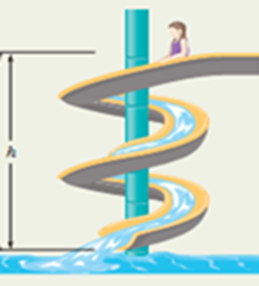
\includegraphics[scale=0.7]{../figs/VN10-2022-PH-TP029-1.png}
			\end{flushright}
		\end{minipage}
	}
	
	\hideall
	{	
		\begin{enumerate}[label=\alph*)]
			\item Tính vận tốc của bạn học sinh khi vừa chạm mặt nước.
			
			Chọn gốc thế năng tại mặt nước. Áp dụng bảo toàn cơ năng:
			$$W_1 = W_2 \Rightarrow 0 + mgz_1 = \dfrac{1}{2}mv_2^2 + 0 \Rightarrow v_2 = \xsi{10\sqrt 2}{m/s}.$$
			\item Ở độ cao nào bạn học sinh có động năng bằng 2 lần thế năng?
			
			Áp dụng bảo toàn cơ năng với $W_\text{đ 3} = 2 W_\text{t 3}$:
			$$W_1 = W_3 \Rightarrow W_1 = 2W_\text{t 3} + W_\text{t 3} = 3 mgz_3 \Rightarrow z_3 = \xsi{10/3}{m}.$$
		\end{enumerate}
	}

	\item \mkstar{3}
	
	
	{
		Từ độ cao $\SI{10}{m}$ người ta thả rơi một vật khối lượng $\SI{2}{kg}$. Bỏ qua lực cản không khí, lấy $g=\SI{10}{m/s^2}$. Tính tốc độ của vật khi động năng của nó lớn hơn thế năng $\SI{60}{J}$.
	}
	
	\hideall
	{	
		Chọn gốc thế năng tại mặt đất. Gọi A, B lần lượt là vị trí thả vật và vị trí có động năng lớn hơn thế năng $\SI{60}{J}$. 
		
		Ta có $W_\text{đ B} = W_\text{t B} + 60 \Rightarrow W_\text{t B} = W_\text{đ B} - 60$.
		
		Áp dụng bảo toàn cơ năng tại A và B:
		$$W_\text{A} = W_\text{B} \Rightarrow 0 + mgz_\text{A} = W_\text{đ B} + (W_\text{đ B} - 60) = 2 W_\text{đ B} - 60 \Rightarrow v_\text{B} = \xsi{\sqrt{130}}{m/s}.$$
	}
	
	\item \mkstar{3}
	
	
	{
		Ở độ cao $\SI{10}{m}$ so với mặt đất, một vật khối lượng $m$ được ném thẳng đứng lên cao với vận tốc $\SI{36}{km/h}$. Chọn gốc thế năng tại mặt đất. Lấy $g=\SI{10}{m/s^2}$.
		\begin{enumerate}[label=\alph*)]
			\item Tính cơ năng của vật và độ cao cực đại mà vật đạt được.
			\item Tại vị trí vật có độ cao $\SI{4}{m}$, tính tỉ số giữa động năng và thế năng của vật.
		\end{enumerate}
	}
	
	\hideall
	{	
		\begin{enumerate}[label=\alph*)]
			\item Tính cơ năng của vật và độ cao cực đại mà vật đạt được.
			
			Cơ năng: $$W_1=\dfrac{1}{2}mv_1^2 + mgz_1 = \SI{15}{J}.$$
			
			Độ cao cực đại (tại $v_2 = 0$):
			$$W_1 = W_2 \Rightarrow \SI{15}{J} = mgz_2 \Rightarrow z_2 = \SI{15}{m}.$$
			
			\item Tại vị trí vật có độ cao $\SI{4}{m}$, tính tỉ số giữa động năng và thế năng của vật.
			
			Thế năng tại $z_3=\SI{4}{m}$:
			$$W_\text{t 3} = mgz_3 = \SI{4}{J}.$$
			
			Động năng tại đó:
			$$W_\text{đ 3} = W - W_\text{t 3} = \SI{11}{J}.$$
			
			Tỉ số động năng và thế năng là $11/4$.
		\end{enumerate}
	}

	\item \mkstar{3}
	
	
	{
		Một con lắc đơn gồm sợi dây nhẹ không dãn, chiều dài $\SI{50}{cm}$, một đầu cố định, đầu còn lại treo vật nặng có khối lượng $\SI{100}{g}$. Ban đầu vật nặng đứng yên ở vị trí cân bằng. Tại vị trí này, truyền cho vật nặng vận tốc $v_0=\SI{5}{m/s}$ theo phương ngang. Chọn gốc thế năng tại vị trí cân bằng và cho $g=\SI{10}{m/s^2}$.
		\begin{enumerate}[label=\alph*)]
			\item Tìm cơ năng của vật.
			\item Khi vật lên đến vị trí M có dây treo hợp với phương thẳng đứng góc $\alpha_\text M$, vật có thế năng bằng $1/4$ động năng. Hãy tính $\alpha_\text M$ và vận tốc của vật tại M.
		\end{enumerate}
	}
	
	\hideall
	{	
		\begin{enumerate}[label=\alph*)]
			\item Tìm cơ năng của vật.
			
			Cơ năng của vật bằng tổng động năng và thế năng:
			$$W_1 = \dfrac{1}{2}mv_1^2 + mgz_1 = \dfrac{1}{2}mv_1^2 + 0 = \SI{1.25}{J}.$$
			
			\item Khi vật lên đến vị trí M có dây treo hợp với phương thẳng đứng góc $\alpha_\text M$, vật có thế năng bằng $1/4$ động năng. Hãy tính $\alpha_\text M$ và vận tốc của vật tại M.
			
			Khi thế năng bằng $1/4$ động năng thì động năng gấp 4 lần thế năng, vậy cơ năng là
			
			$$W_2 = W_\text{đ 2} + W_\text{t 2} = 4 W_\text{t 2} + W_\text{t 2} = 5 W_\text{t 2} = W_1 \Rightarrow 5mgz_2 = \SI{1.25}{J} \Rightarrow z_2 = \SI{0.25}{m}.$$
			
			Mà góc $\alpha_\text M$ giữa phương thẳng đứng và phương dây treo được tính theo công thức: $\cos \alpha_\text M = \dfrac{l-z_2}{l} = \dfrac{1}{2}$, suy ra $\alpha_\text M = 60^\circ$.
			
			Vận tốc của vật tại M:
			$$W_\text{đ 2} = 4 W_\text{t 2} \Rightarrow \dfrac{1}{2}mv_2^2 = 4 mgz_2 \Rightarrow v_2 = \xsi{2\sqrt 5}{m/s}.$$
		\end{enumerate}
	}
	
	\item \mkstar{3}
	
	
	{
		Thả rơi không vận tốc đầu một vật có khối lượng $m=\SI{200}{g}$ từ độ cao $h_0=\SI{5}{m}$ so với mặt đất. Lấy $g=\SI{10}{m/s^2}$ và bỏ qua mọi lực cản.
		\begin{enumerate}[label=\alph*)]
			\item Tính cơ năng của vật và tốc độ của vật khi vừa chạm đất.
			\item Tính thế năng và động năng của vật khi vật có động năng bằng 3 lần thế năng. Khi đó vật có tốc độ và độ cao bao nhiêu?
			\item Kể từ lúc thả, sau thời gian ngắn nhất bao lâu thì vật có thế năng bằng 3 lần động năng?
		\end{enumerate}
	}
	
	\hideall
	{	
		\begin{enumerate}[label=\alph*)]
			\item Tính cơ năng của vật và tốc độ của vật khi vừa chạm đất.
			
			Cơ năng:
			$$W_1 = mgh_0 + 0 = \SI{10}{J}.$$
			
			Khi vật chạm đất:
			$$W_1 = W_2 \Rightarrow \SI{10}{J} = \dfrac{1}{2} mv_2^2 + 0 \Rightarrow v_2 = \SI{10}{m/s}.$$
			
			\item Tính thế năng và động năng của vật khi vật có động năng bằng 3 lần thế năng. Khi đó vật có tốc độ và độ cao bao nhiêu?
			
			Ta có $W_\text{đ 3} = 3 W_\text{t 3}$ nên $W_3 = 4 W_\text{t 3} = \SI{10}{J}$, suy ra $W_\text{t 3} = \SI{2.5}{J}$, $z_3 = \SI{1.25}{m}$.
			
			Và $W_\text{đ 3} = \SI{7.5}{J}$, $v_3 = \xsi{5\sqrt 3}{m/s}$.
			
			\item Kể từ lúc thả, sau thời gian ngắn nhất bao lâu thì vật có thế năng bằng 3 lần động năng?
			
			Khi $W_\text{t 4} = 3W_\text{đ 4}$ thì $W_4 = \dfrac{4}{3} W_\text{t 4} = \dfrac{4}{3} mgz_4$, suy ra $z_4 = \SI{3.75}{m}$.
			
			Quãng đường vật rơi được: $s=h_0-z_4 = \SI{1.25}{m}$. Áp dụng công thức:
			$$s=\dfrac{1}{2}gt^2 \Rightarrow t = \SI{5}{s}.$$
		\end{enumerate}
	}
	
	\item \mkstar{3}
	
	
	{
		Vật nặng $\SI{2}{kg}$ trượt không vận tốc đầu từ đỉnh A của cung AB là $1/4$ cung tròn bán kính $R=\SI{2.4}{m}$. Sau đó tiếp tục trượt trên mặt ngang BC cách mặt đất độ cao $h=\SI{2}{m}$. Cho $g=\SI{10}{m/s^2}$. Bỏ qua ma sát, áp dụng dụng định luật bảo toàn cơ năng.
		\begin{enumerate}[label=\alph*)]
			\item Tính vận tốc của vật tại C.
			\item Đến C vật rơi ngang và rơi xuống đất. Tính vận tốc của vật khi vật chạm đất.
		\end{enumerate}
		\begin{center}
			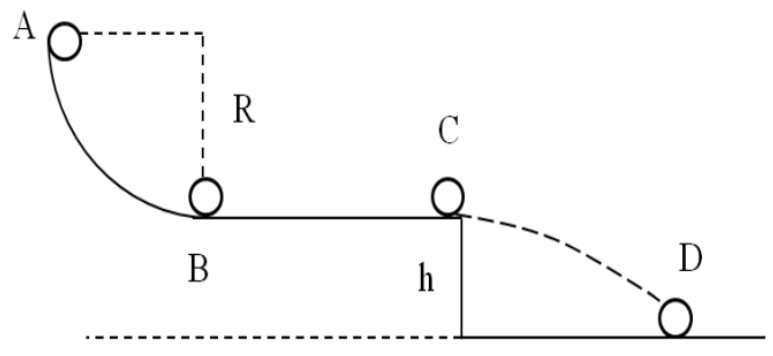
\includegraphics[scale=0.4]{../figs/VN10-2022-PH-TP029-4}
		\end{center}
	}
	
	\hideall
	{	
		\begin{enumerate}[label=\alph*)]
			\item Tính vận tốc của vật tại C.
			
			Chọn gốc thế năng tại mặt đất (tại D).
			
			Độ cao điểm A là $z_\text{A} = h + R = \SI{4.4}{m}$.
			
			Độ cao điểm C là $z_\text{C} = h = \SI{2}{m}$.
			
			Áp dụng bảo toàn cơ năng tại A và C:
			$$W_\text{A} = W_\text{C} \Rightarrow 0 + mgz_\text A = \dfrac{1}{2}mv_\text{C}^2 + mgz_\text{C} \Rightarrow v_\text{C} = \xsi{4\sqrt 3}{m/s}.$$
			
			\item Đến C vật rơi ngang và rơi xuống đất. Tính vận tốc của vật khi vật chạm đất.
			
			Áp dụng bảo toàn cơ năng tại C và D, với $z_\text{D} = 0$:
			$$W_\text{C} = W_\text{D} \Rightarrow \dfrac{1}{2}mv_\text{C}^2 + mgz_\text{C} = \dfrac{1}{2} mv_\text{D}^2 + 0 \Rightarrow v_\text{D} = \xsi{2\sqrt{22}}{m/s}.$$
		\end{enumerate}
	}
	
	
	
	\item \mkstar{3}
	
	
	{
		Một viên bi nhỏ khối lượng $\SI{200}{g}$ được ném thẳng đứng xuống dưới từ điểm O có độ cao $\SI{7}{m}$ so với mặt đất với tốc độ ban đầu $\SI{4}{m/s}$. Bỏ qua sức cản của không khí, lấy $g=\SI{10}{m/s^2}$. Giải bài toán bằng phương pháp năng lượng, chọn gốc thế năng tại mặt đất. Đất mềm, viên bi lún thẳng xuống mặt đất thêm một đoạn $\SI{10}{cm}$. Tính lực cản trung bình của đất tác dụng lên viên bi.
	}
	
	\hideall
	{	
		Cơ năng của vật tại ví trí ném:
		$$W_1 = W_\text{đ 1} + W_\text{t 1} = \SI{15.6}{J}.$$
		
		Cơ năng của vật tại vị trí sâu $\SI{10}{cm}$ dưới đất:
		$$W_2 = 0 + mgz_2 = \SI{-0.2}{J}.$$
		
		Khi vật dừng lại thì toàn bộ cơ năng chuyển thành công của lực cản của đất:
		$$\Delta W = W_2 - W_1 = \SI{-15.8}{J}= A_\text{cản} = -F_\text{c} \cdot \SI{0.1}{m} \Rightarrow F_\text{cản} = \SI{158}{N}.$$
	}
	\item \mkstar{3}
	
	
	{
		Một vật có khối lượng $\SI{2}{kg}$ được thả rơi tự do từ độ cao $\SI{2.5}{m}$ so với mặt đất. Lấy $g=\SI{10}{m/s^2}$, bỏ qua mọi lực cản của không khí. Chọn gốc thế năng ở mặt đất.
		
		Khi rơi đến mặt đất, vật va chạm với mặt đất và nảy lên đến độ cao cực đại là $\SI{2}{m}$. Tìm phần cơ năng đã mất đi sau khi vật va chạm với mặt đất.
	}
	
	\hideall
	{	
		Cơ năng lúc thả vật (cơ năng trước khi vật va chạm với mặt đất):
		$$W_1 = mgz_1 = \SI{50}{J}.$$
		
		Cơ năng lúc vật nảy lên đến độ cao cực đại (cơ năng sau khi vật va chạm với mặt đất):
		$$W_2 = mgz_2 = \SI{40}{J}.$$
		
		Phần cơ năng đã mất đi: $$\Delta W = |W_2 - W_1| = \SI{10}{J}.$$
	}
	
	\item \mkstar{3}
	
	
	{
		Ném một vật thẳng đứng lên trên với vận tốc $\SI{5}{m/s}$ từ độ cao $\SI{1.5}{m}$ so với mặt đất. Bỏ qua mọi lực cản, cho $g=\SI{10}{m/s^2}$.
		\begin{enumerate}[label=\alph*)]
			\item Tính độ cao cực đại mà vật đạt được và quãng đường mà vật đi được từ khi đạt độ cao cực đại đến khi vật có thế năng bằng 4 lần động năng.
			\item Khi vật đến mặt đất tại điểm D, do đất mềm nên vật lún vào đất $\SI{20}{cm}$. Tính công của lực cản trung bình của đất tác dụng lên vật. Biết khối lượng vật bằng $\SI{400}{g}$.
		\end{enumerate}
	}
	
	\hideall
	{	
		\begin{enumerate}[label=\alph*)]
			\item Tính độ cao cực đại mà vật đạt được và quãng đường mà vật đi được từ khi đạt độ cao cực đại đến khi vật có thế năng bằng 4 lần động năng.
			
			Chọn gốc thế năng tại mặt đất. Áp dụng bảo toàn cơ năng tại vị trí ném và vị trí độ cao cực đại:
			$$W_\text{A} = W_\text{B} \Rightarrow \dfrac{1}{2}mv_\text{A}^2 + mgz_\text{A} = 0 + mgz_\text{B} \Rightarrow z_\text{B} = \SI{2.75}{m}.$$
			
			Khi vật có thế năng bằng 4 lần động năng $W_\text{t C} = 4 W_\text{đ C}$ thì $W_\text{C} = \dfrac{W_\text{t C}}{4} + W_\text{C} = \dfrac{5 W_\text{t C}}{4}$. Áp dụng bảo toàn cơ năng:
			$$W_\text{A} = W_\text{C} \Rightarrow \dfrac{1}{2}mv_\text{A}^2 + mgz_\text{A} = \dfrac{5 mgz_\text{C}}{4}  \Rightarrow z_\text{C} = \SI{2.2}{m}.$$
			
			Vậy quãng đường vật đi được từ khi đạt độ caoc cực đại đến khi vật có thế năng bằng 4 lần động năng là $s=z_\text{B} - z_\text{C} = \SI{0.55}{m}$.
			
			\item Khi vật đến mặt đất tại điểm D, do đất mềm nên vật lún vào đất $\SI{20}{cm}$. Tính công của lực cản trung bình của đất tác dụng lên vật. Biết khối lượng vật bằng $\SI{400}{g}$.
			
			Cơ năng tại điểm D có $z_\text{D} = \SI{-0.2}{m}$: $W_\text{D} = mgz_\text{D} = \SI{-0.8}{J}$
			
			Độ biến thiên cơ năng bằng công của lực cản:
			$$A_\text{cản} = \Delta W = W_\text{D} - W_\text{A} = \SI{-11.8}{J}.$$
		\end{enumerate}
	}
	
	\item \mkstar{3}
	
	
	{
		Từ tầng 10 của tòa nhà cao tầng cách mặt đất $\SI{35}{m}$, một vật nặng $\SI{200}{g}$ được ném theo phương thẳng đứng, hướng xuống với tốc độ $\SI{20}{m/s}$. Chọn mốc thế năng tại mặt đất, bỏ qua mọi ma sát và lực cản của không khí, lấy $g=\SI{10}{m/s^2}$. Khi rơi xuống đất, do đất mềm và lún thì người ta thấy vật lún sâu vào đất một đoạn. Biết lực cản trung bình của đất là $\SI{440}{N}$. Tìm độ sâu vật lún vào đất.
	}
	
	\hideall
	{	
		Cơ năng lúc ném vật:
		$$W_1 = \dfrac{1}{2}mv_1^2 + mgz_1 = \SI{110}{J}.$$
		
		Cơ năng vật lúc vật ở độ sâu $d$ trong đất:
		$$W_2 = -mgd.$$
		
		Độ biến thiên cơ năng bằng công của lực cản:
		$$W_2 - W_1 = -F_\text{c} d \Rightarrow -mgd - W_1 = -F_\text{c} d \Rightarrow d = \SI{0.25}{m}.$$
		
		Vậy độ sâu vật lún vào đất là $d=\SI{0.25}{m}$.
	}
	\item \mkstar{3}
	
	
	{
		Một vật trượt không vận tốc đầu từ đỉnh mặt phẳng nghiêng cao $\SI{1.25}{m}$. Cho gia tốc rơi tự do $g=\SI{10}{m/s^2}$.
		\begin{enumerate}[label=\alph*)]
			\item Vật trượt không ma sát trên mặt phẳng nghiêng. Hãy tính vận tốc của vật tại chân mặt phẳng nghiêng.
			\item Khi đến chân mặt phẳng nghiêng, vật tiếp tục trượt trên mặt phẳng nằm ngang nối liền với mặt nghiêng. Thời gian chuyển động của vật trên mặt phẳng ngang là $\SI{5}{s}$. Tính hệ số ma sát giữa vật và mặt phẳng nằm ngang.
		\end{enumerate}
	}
	
	\hideall
	{	
		\begin{enumerate}[label=\alph*)]
			\item Vật trượt không ma sát trên mặt phẳng nghiêng. Hãy tính vận tốc của vật tại chân mặt phẳng nghiêng.
			
			Chọn gốc thế năng tại mặt đất. Bảo toàn cơ năng tại đỉnh dốc và chân dốc:
			$$W_1 = W_2 \Rightarrow 0 + mgz_1 = \dfrac{1}{2}mv_2^2 + 0 \Rightarrow v_2 = \SI{5}{m/s}.$$
			
			\item Khi đến chân mặt phẳng nghiêng, vật tiếp tục trượt trên mặt phẳng nằm ngang nối liền với mặt nghiêng. Thời gian chuyển động của vật trên mặt phẳng ngang là $\SI{5}{s}$. Tính hệ số ma sát giữa vật và mặt phẳng nằm ngang.
			
			Gia tốc của vật trên mặt nghiêng:
			$$v_3 = 0 = at + v_2 \Rightarrow a = \SI{-1}{m/s^2}.$$
			
			Quãng đường vật trượt trên mặt ngang:
			$$s=\dfrac{1}{2}at^2 + v_2 t = \SI{12.5}{m}.$$
			
			Độ biến thiên cơ năng bằng công của lực ma sát:
			$$W_3 - W_2 = -\mu mg s \Rightarrow 0 - \dfrac{1}{2}mv_2^2 = -\mu mg s \Rightarrow \mu = \SI{0.1}{}.$$	
			
		\end{enumerate}
	}

\end{enumerate}